\documentclass{beamer}
\usepackage{../common_slides}
\usepackage{tikz}
\usepackage{pdfpages}

\usetikzlibrary{matrix}
% \usepackage{enumitem}
\tikzstyle{hid}=[draw]
\tikzstyle{obs}=[draw]

\title{Machine Translation 2 \\ Neural Machine Translation}
\date{}
\author{CS 287}

\begin{document}
\begin{frame}
  \titlepage
\end{frame}


\begin{frame}{Review: Simple One-to-One Model}
  \begin{enumerate}
  \item Language Model; words depend on previous word
    \[ p(\boldy) = \prod_{i=1}^n p(\boldy_i | \boldy_{i-1})  \] 
    \air 

  \item Translation Model; source word depends on current position
    \[ p(\boldx | \boldy) = \prod_{i=1}^n p(\boldx_i | \boldx_{i-1})  \] 
  \end{enumerate}

  % What model is this?
\end{frame}

\begin{frame}{Review: Alignment}
  \begin{itemize}
  \item $\bolda$; alignment mapping each target word to a source word
  \item Assuming one-to-one
  \end{itemize}


  \begin{center}
    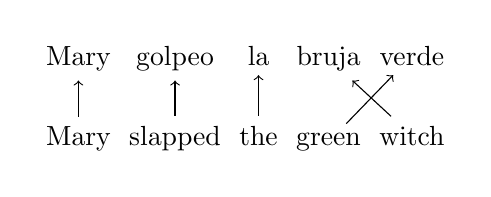
\begin{tikzpicture}
    \matrix(dict)[matrix of nodes, ampersand replacement=\&]{
      Mary \& golpeo \& la \& bruja \& verde \\
      ~\\
      ~\\
      Mary \& slapped \& the \& green \& witch  \\ };
    \path[draw, <-] (dict-1-1) -> (dict-4-1);
    \path[draw, <-] (dict-1-2) -> (dict-4-2);
    \path[draw, <-] (dict-1-3) -> (dict-4-3);
    \path[draw, <-] (dict-1-4) -> (dict-4-5);
    \path[draw, <-] (dict-1-5) -> (dict-4-4);
  \end{tikzpicture}
  \end{center}
  \begin{center}
  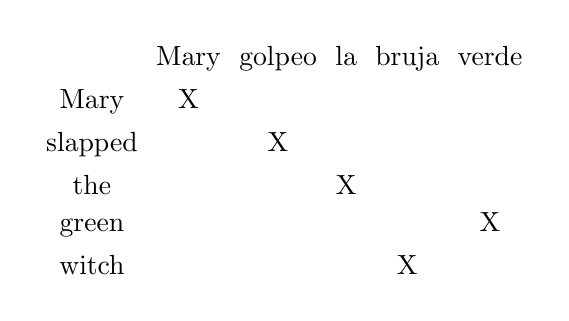
\begin{tikzpicture}
    \matrix(dict)[matrix of nodes, ampersand replacement=\&]{
      \ \& Mary \& golpeo \& la \& bruja \& verde \\
      Mary \& X \&  \&  \&  \&  \\
      slapped \&  \& X \&  \&  \&  \\
      the \&  \&  \&  X\&  \&  \\
      green \&  \&  \&  \&  \& X \\
      witch \&  \&  \&  \& X  \&  \\
    };
    \end{tikzpicture}
  \end{center}
\end{frame}


\begin{frame}{Review: Using Alignments}
  \[ p(\boldy | \boldx) \propto \sum_{\bolda} p(\boldy) p(\bolda | \boldy) p(\boldx |  \bolda, \boldy)  \]  

  With alignment,
  \[ p(\boldx |  \bolda, \boldy)  = \prod_{i=1}^n p(\boldx_{a_i} | \boldy_i) \] 

  \air 

  Sum-over-alignment approximated with a max-over-alignment,

  \[ \argmax_{j, w^t_{1:n}} \prod_{i=1}^n p(\boldx_{a_i} | \boldy_i=w^t_i) p(\boldy_i=w^t_i | \boldy_{i-1}=w^t_{i-1}) p(a_i = c_i | a_{i-1}=c_{i-1}, i)   \]  
\end{frame}

\begin{frame}{Quiz: CRF}
  Note: Nothing in our definition of CRFs relied on $\boldy_i$ to align
  with $\boldx_i$ (conditioned on full sequence). 

  For this quiz, imagine we have an input sequence $\boldx$, and we want to 
  find the optimal output sequence $\boldy$ but we do not fix $n < N$. For instance 
  finding the best word segmentation of an unsegmented input $\boldx$. 

  \begin{itemize}
  \item How would you find \[ \argmax_{n, c_{1:n}} f(\boldx, c_{1,n}) ?\]

  \item How would you train \[ f(\boldx, c_{1,n}; \theta) ?\] 
  \end{itemize}
\end{frame}

\begin{frame}{Preliminaries}
  \begin{itemize}
  \item How alignment is used in SMT.
    \air

  \item Language Model RNNs 
  \item Bidirectional RNNs 
  \item Stacked RNNs 
  \end{itemize}
\end{frame}

\begin{frame}{Bit-Set Beam Search}
  [Describe on board] 
\end{frame}

\begin{frame}{Stacked RNN}
  \begin{center}
    \includegraphics[width=10cm]{deeprnn}
  \end{center}
\end{frame}


\begin{frame}{RNN for Language Modeling}
  \begin{itemize}
  \item Recent popularization of RNNs has been based on language modeling (Mikolov, 2012)
    \air

  \item In particular RNNs allow for non-Markovian models
    \[ p(w_i | w_1, \ldots, w_{i-1};\theta) = O(\bolds_i) \]

    \air 

  \item Compare this to the feed-forward windowed approach.
    \[ p(w_i | w_{i-n+1}, \ldots, w_{i-1};\theta) = O(\bolds_i) \]
  \end{itemize}
\end{frame}


\begin{frame}{RNN as Transducer}
  \begin{center}
  \begin{tikzpicture}
    \node(ya){$\hat{\boldy}_1$}; 

    \node(sa)[below=of ya]{$\bolds_1$}; 
    \node(xa)[below=of sa]{$\boldx_1$}; 
    \node(yb)[right=of ya]{$\hat{\boldy}_2$}; 
    \node(sb)[below=of yb]{$\bolds_2$}; 
    \node(xb)[below=of sb]{$\boldx_2$}; 
    \node(yc)[right=of yb]{$\hat{\boldy}_3$}; 
    \node(sc)[below=of yc]{$\bolds_3$}; 
    \node(xc)[below=of sc]{$\boldx_3$}; 
    \draw (sa) edge (sb); 
    \draw (sb) edge (sc); 


    \draw (sa) -- (xa); 
    \draw (sb) -- (xb); 
    \draw (sc) -- (xc); 
    \draw (sa) -- (ya); 
    \draw (sb) -- (yb); 
    \draw (sc) -- (yc); 
  \end{tikzpicture}
  \end{center}
  \begin{itemize}
  \item Can reuse hidden state each time
    \[ p(w_i | w_1, \ldots, w_{i-1};\theta) = O(\bolds_i) = O(R(\bolds_{i-1}, \boldx_{i})) \]
    \[ p(w_{i+1} | w_1, \ldots, w_{i};\theta) = O(R(\bolds_{i}, \boldx_{i+1})) \]
  \end{itemize}
\end{frame}


\begin{frame}{Bidirectional Models}
  \begin{itemize}
    \item For all $i \in \{1, \ldots, n \}$ 

      \[\bolds^f_{i} = R^{f}(\bolds_{i-1}, \boldx_i) \]

    \item For all $i \in \{1, \ldots, n \}$ 

      \[\bolds^b_{i} = R^{b}(\bolds_{i+1}, \boldx_i) \]

    \item For all $i \in \{1, \ldots, n \}$ 
      \[ \hat{\boldy}_i = O([\bolds^b_{i}, \bolds^f_{i}]) = [\bolds^b_{i}, \bolds^f_{i}] \boldW + \boldb \] 
  \end{itemize}
\end{frame}

\begin{frame}
  \begin{center}
    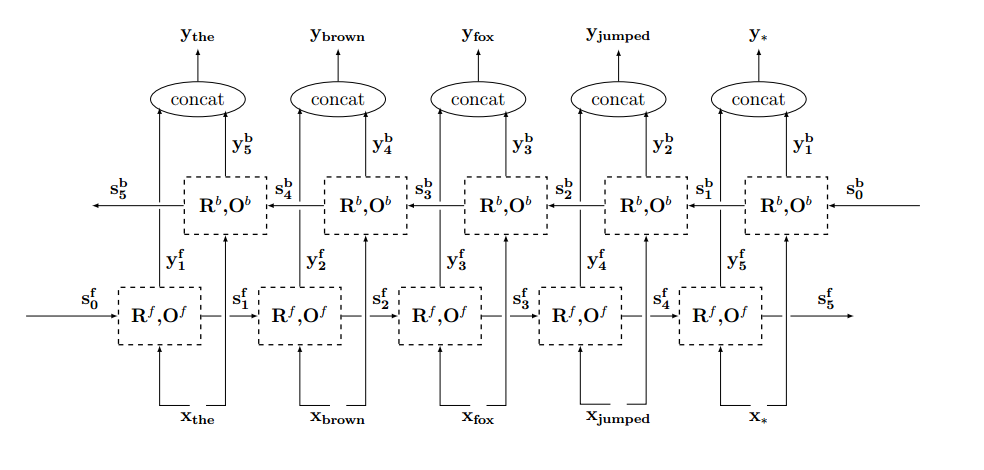
\includegraphics[width=10cm]{ygbidirection}
  \end{center}
\end{frame}


\begin{frame}{Today's Lecture}
  \begin{enumerate}
  \item Sequence-to-Sequence Model (Sutskever et al 2014)
    \air
  \item Attention-Based Model (Bahdanau et al 2014)
  \end{enumerate}
\end{frame}

\section{Sequence-To-Sequence}



\begin{frame}{Neural Machine Translation}
  \begin{itemize}
  \item $\boldx  = [ w^s_1\ w^s_2\ w^s_3\ldots w^s_n $] 
  \item $\boldy =  [w^t_1\ w^t_2\ w^t_3\ldots w^t_n $] 
  \end{itemize}

 
  \[ p(w^t | w^s) = \prod_{i=1}^n p(w^t_i | w^s, \theta)  \] 

  Intuition:

  \begin{enumerate}
  \item Start with bag-of-source words
  \item Pick a source word, translate it to a target word that ``fits''
  \item Update source bag representation.
  \end{enumerate}
\end{frame}


% \begin{frame}{Babbler}
%   \begin{itemize}
%   \item \[ p(w_i | w_1, \ldots, w_{i-1}) = \softmax(RNN()) = \hat{y}_{w_i}   \] 
%   \end{itemize}
% \end{frame}

\begin{frame}{Encoder-Decoder Idea}
  Compute a single vector $\bolds^t$ encoding 
  the source. 
  
  \begin{itemize}
  \item \[ p(w^t_i | w^t_1, \ldots, w^t_{i-1}, \bolds) = \hat{y}_{w_i}   \] 
  \end{itemize}

  Intuition:

  \begin{itemize}
  \item Start with encoded source 
  \item Use encoded vector to translate to a target word that ``fits''
  \item Update source representation
  \end{itemize}
\end{frame}


\begin{frame}{Encoder}
  \begin{itemize}
  \item How do you get a source encoding? LSTM (or bi-LSTM)
    \air 
  \end{itemize}
    
  \begin{center}
    \begin{tikzpicture}
      \matrix (network) [matrix of nodes, ampersand replacement=\&,
      column sep={1cm},
      row sep={1cm}] {
        \& \&   \\
        \& \&  \node{$\hat{\boldy}$}; \\
        \node[hid]{$\bolds^s_1$}; \& \node[hid]{$\bolds^s_2$}; \& \node[hid]{$\bolds^s_3$}; \\
        \node[obs]{$\boldx_1$}; \& \node[obs]{$\boldx_2$}; \& \node[obs]{$\boldx_3$};  \\
          \node[obs]{the}; \& \node[obs]{red}; \& \node[obs]{dog};  \\
      }; 


      \draw[->] (network-5-1) -- (network-4-1); 
      \draw[->] (network-5-2) -- (network-4-2); 
      \draw[->] (network-5-3) -- (network-4-3);


      \draw[->] (network-4-1) -- (network-3-1); 
      \draw[->] (network-4-2) -- (network-3-2); 
      \draw[->] (network-4-3) -- (network-3-3);


      \draw[->] (network-3-1.east) -- (network-3-2.west); 
      \draw[->] (network-3-2.east) -- (network-3-3.west); 
      \draw[->] (network-3-3) -- (network-2-3); 
    \end{tikzpicture}
  \end{center}  
\end{frame}



\begin{frame}{Decoder}
  \begin{itemize}
  \item How do you use this source encoding? LSTM 
  \end{itemize}


  \begin{center}
    \begin{tikzpicture}
      \matrix (network) [matrix of nodes, ampersand replacement=\&,
      column sep={1cm},
      row sep={1cm}] {
        \& \& \& \node{the}; \& \node{red}; \& \node{dog}; \\
        \& \& \& \node[obs]{$\hat{\boldy}_1$}; \& \node[obs]{$\hat{\boldy}_2$}; \& \node[obs]{$\hat{\boldy}_3$}; \\
        \&  \&  \& \node[hid]{$\bolds^t_1$}; \& \node[hid]{$\bolds^t_2$}; \& \node[hid]{$\bolds^t_3$}; \\
         \&  \&   \&   \node[obs]{$\hat{\boldx}_1$}; \& \node[obs]{$\hat{\boldx}_2$}; \& \node[obs]{$\hat{\boldx}_3$}; \\
           \&  \&   \&  \node[obs]{$<$s$>$}; \&  \&  \\
      }; 



      \draw[->] (network-5-4) -- (network-4-4);
      \draw[->] (network-1-4) -- (network-4-5.west); 
      \draw[->] (network-1-5) -- (network-4-6.west); 

      \draw[->] (network-3-4.east) -- (network-3-5.west); 
      \draw[->] (network-3-5.east) -- (network-3-6.west); 

      \draw[->] (network-2-4) -- (network-1-4); 
      \draw[->] (network-2-5) -- (network-1-5); 
      \draw[->] (network-2-6) -- (network-1-6);

      \draw[->] (network-4-4) -- (network-3-4); 
      \draw[->] (network-4-5) -- (network-3-5); 
      \draw[->] (network-4-6) -- (network-3-6);

      \draw[->] (network-3-4) -- (network-2-4); 
      \draw[->] (network-3-5) -- (network-2-5); 
      \draw[->] (network-3-6) -- (network-2-6);

    \end{tikzpicture}
  \end{center}  
\end{frame}


\begin{frame}{Sequence-to-Sequence}
  \begin{center}
    \begin{tikzpicture}
      \matrix (network) [matrix of nodes, ampersand replacement=\&,
      column sep={1cm},
      row sep={1cm}] {
        \& \& \& \node{the}; \& \node{red}; \& \node{dog}; \\
        \& \& \& \node[obs]{$\hat{\boldy}_1$}; \& \node[obs]{$\hat{\boldy}_2$}; \& \node[obs]{$\hat{\boldy}_3$}; \\
        \node[hid]{$\bolds^s_1$}; \& \node[hid]{$\bolds^s_2$}; \& \node[hid]{$\bolds^s_3$}; \& \node[hid]{$\bolds^t_1$}; \& \node[hid]{$\bolds^t_2$}; \& \node[hid]{$\bolds^t_3$}; \\
        \node[obs]{$\boldx_1$}; \& \node[obs]{$\boldx_2$}; \& \node[obs]{$\boldx_3$};  \&   \node[obs]{$\hat{\boldx}_1$}; \& \node[obs]{$\hat{\boldx}_2$}; \& \node[obs]{$\hat{\boldx}_3$}; \\
        \node[obs]{the}; \& \node[obs]{red}; \& \node[obs]{dog};  \&  \node[obs]{$<$s$>$}; \&  \&  \\
      }; 


      \draw[->] (network-5-1) -- (network-4-1); 
      \draw[->] (network-5-2) -- (network-4-2); 
      \draw[->] (network-5-3) -- (network-4-3);
      \draw[->] (network-5-4) -- (network-4-4);


      \draw[->] (network-4-1) -- (network-3-1); 
      \draw[->] (network-4-2) -- (network-3-2); 
      \draw[->] (network-4-3) -- (network-3-3);


      \draw[->] (network-3-1.east) -- (network-3-2.west); 
      \draw[->] (network-3-2.east) -- (network-3-3.west); 
      \draw[->] (network-3-3.east) -- (network-3-4.west); 



      
      \draw[->] (network-1-4) -- (network-4-5.west); 
      \draw[->] (network-1-5) -- (network-4-6.west); 

      \draw[->] (network-3-4.east) -- (network-3-5.west); 
      \draw[->] (network-3-5.east) -- (network-3-6.west); 

      \draw[->] (network-2-4) -- (network-1-4); 
      \draw[->] (network-2-5) -- (network-1-5); 
      \draw[->] (network-2-6) -- (network-1-6);

      \draw[->] (network-4-4) -- (network-3-4); 
      \draw[->] (network-4-5) -- (network-3-5); 
      \draw[->] (network-4-6) -- (network-3-6);

      \draw[->] (network-3-4) -- (network-2-4); 
      \draw[->] (network-3-5) -- (network-2-5); 
      \draw[->] (network-3-6) -- (network-2-6);

    \end{tikzpicture}
  \end{center}
\end{frame}



\begin{frame}{Stacked Sequence-to-Sequence}
  \begin{center}
    \begin{tikzpicture}
      \matrix (network) [matrix of nodes, ampersand replacement=\&,
      column sep={1cm},
      row sep={1cm}] {
        \& \& \& \node{the}; \& \node{red}; \& \node{dog}; \\
        \& \& \& \node[obs]{$\hat{\boldy}_1$}; \& \node[obs]{$\hat{\boldy}_2$}; \& \node[obs]{$\hat{\boldy}_3$}; \\
        \node[hid]{$\bolds^s_1$}; \& \node[hid]{$\bolds^s_2$}; \& \node[hid]{$\bolds^s_3$}; \& \node[hid]{$\bolds^t_1$}; \& \node[hid]{$\bolds^t_2$}; \& \node[hid]{$\bolds^t_3$}; \\
        \node[hid]{$\bolds^s_1$}; \& \node[hid]{$\bolds^s_2$}; \& \node[hid]{$\bolds^s_3$}; \& \node[hid]{$\bolds^t_1$}; \& \node[hid]{$\bolds^t_2$}; \& \node[hid]{$\bolds^t_3$}; \\
        \node[obs]{$\boldx_1$}; \& \node[obs]{$\boldx_2$}; \& \node[obs]{$\boldx_3$};  \&   \node[obs]{$\hat{\boldx}_1$}; \& \node[obs]{$\hat{\boldx}_2$}; \& \node[obs]{$\hat{\boldx}_3$}; \\
          \node[obs]{the}; \& \node[obs]{red}; \& \node[obs]{dog};  \&  \node[obs]{$<$s$>$}; \&  \&  \\
      }; 


      \draw[->] (network-6-1) -- (network-5-1); 
      \draw[->] (network-6-2) -- (network-5-2); 
      \draw[->] (network-6-3) -- (network-5-3);
      \draw[->] (network-6-4) -- (network-5-4);


      \draw[->] (network-4-1) -- (network-3-1); 
      \draw[->] (network-4-2) -- (network-3-2); 
      \draw[->] (network-4-3) -- (network-3-3);

      \draw[->] (network-5-1) -- (network-4-1); 
      \draw[->] (network-5-2) -- (network-4-2); 
      \draw[->] (network-5-3) -- (network-4-3);


      \draw[->] (network-3-1.east) -- (network-3-2.west); 
      \draw[->] (network-3-2.east) -- (network-3-3.west); 
      \draw[->] (network-3-3.east) -- (network-3-4.west); 

      \draw[->] (network-4-1.east) -- (network-4-2.west); 
      \draw[->] (network-4-2.east) -- (network-4-3.west); 
      \draw[->] (network-4-3.east) -- (network-4-4.west); 



      
      \draw[->] (network-1-4) -- (network-5-5.west); 
      \draw[->] (network-1-5) -- (network-5-6.west); 

      \draw[->] (network-3-4.east) -- (network-3-5.west); 
      \draw[->] (network-3-5.east) -- (network-3-6.west); 

      \draw[->] (network-4-4.east) -- (network-4-5.west); 
      \draw[->] (network-4-5.east) -- (network-4-6.west); 


      \draw[->] (network-2-4) -- (network-1-4); 
      \draw[->] (network-2-5) -- (network-1-5); 
      \draw[->] (network-2-6) -- (network-1-6);

      \draw[->] (network-4-4) -- (network-3-4); 
      \draw[->] (network-4-5) -- (network-3-5); 
      \draw[->] (network-4-6) -- (network-3-6);

      \draw[->] (network-5-4) -- (network-4-4); 
      \draw[->] (network-5-5) -- (network-4-5); 
      \draw[->] (network-5-6) -- (network-4-6);


      \draw[->] (network-3-4) -- (network-2-4); 
      \draw[->] (network-3-5) -- (network-2-5); 
      \draw[->] (network-3-6) -- (network-2-6);

    \end{tikzpicture}
  \end{center}
\end{frame}

\begin{frame}{Paper}
  \begin{center}
    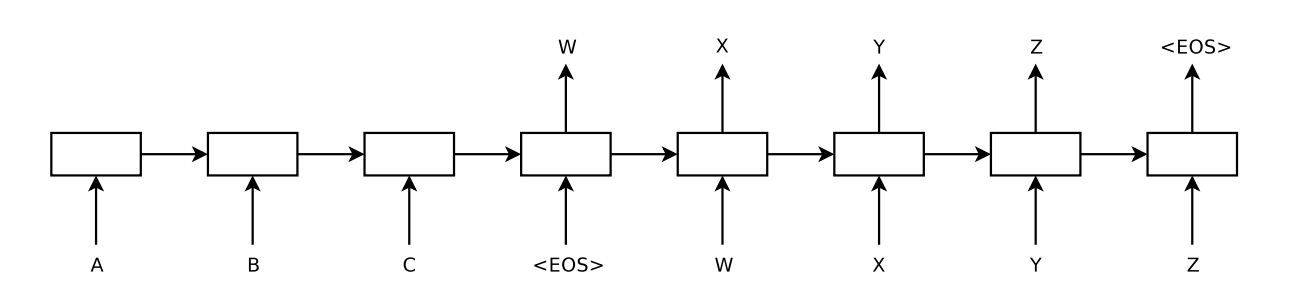
\includegraphics[width=10cm]{seq2seq}
  \end{center}
\end{frame}

\begin{frame}
  \begin{quote}
    While the LSTM is capable of solving problems with long term
    dependencies, we discovered that the LSTM learns much better when
    the source sentences are reversed (the target sentences are not
    reversed). By doing so, the LSTM’s test perplexity dropped from
    5.8 to 4.7, and the test BLEU scores of its decoded translations
    increased from 25.9 to 30.6.
  \end{quote}
\end{frame}

% \begin{frame}
  
% \end{frame}


\begin{frame}
  \begin{quote}
    We found that the LSTM models are fairly easy to train. We used
    deep LSTMs with 4 layers, with 1000 cells at each layer and 1000
    dimensional word embeddings, with an input vocabulary of 160,000
    and an output vocabulary of 80,000. We found deep LSTMs to
    significantly outperform shallow LSTMs, where each additional
    layer reduced perplexity by nearly 10\%, possibly due to their
    much larger hidden state. We used a naive softmax over 80,000
    words at each output. The resulting LSTM has 380M parameters of
    which 64M are pure recurrent connections (32M for the “encoder”
    LSTM and 32M for the “decoder” LSTM). The complete training
    details are given below:
  \end{quote}
\end{frame}

\begin{frame}
  \begin{quote}
    We search for the most likely translation using a simple left-to-right beam search decoder which
maintains a small number B of partial hypotheses, where a partial hypothesis is a prefix of some
translation. At each timestep we extend each partial hypothesis in the beam with every possible
word in the vocabulary. This greatly increases the number of the hypotheses so we discard all but
the B most likely hypotheses according to the model’s log probability. As soon as the EOS
symbol is appended to a hypothesis, it is removed from the beam and is added to the set of complete
hypotheses. While this decoder is approximate, it is simple to implement. Interestingly, our system
performs well even with a beam size of 1, and a beam of size 2 provides most of the benefits of beam
search (Table 1).
  \end{quote}
\end{frame}

\begin{frame}{Paper}
  \begin{center}
    \includegraphics[width=10cm]{seqres}
  \end{center}
\end{frame}


\section{Attention-Based}

\begin{frame}{Sequence-To-Sequence}
  \begin{itemize}
  \item True Encoder-Decoder stores full sentence in single vector.
    \air 
  \item In practice we have access to the original at decoding time. 
   
  \end{itemize}
\end{frame}


\begin{frame}
  \begin{center}
    \begin{tikzpicture}
      \matrix (network) [matrix of nodes, ampersand replacement=\&,
      column sep={1cm},
      row sep={1cm}] {
        \& \& \& \node{the}; \& \node{red}; \& \node{dog}; \\
        \& \& \& \node[obs]{$\hat{\boldy}_1$}; \& \node[obs]{$\hat{\boldy}_2$}; \& \node[obs]{$\hat{\boldy}_3$}; \\
        \node[hid]{$\bolds^s_1$}; \& \node[hid]{$\bolds^s_2$}; \& \node[hid]{$\bolds^s_3$}; \& \node[hid]{$\bolds^t_1$}; \& \node[hid]{$\bolds^t_2$}; \& \node[hid]{$\bolds^t_3$}; \\
        \node[hid]{$\bolds^s_1$}; \& \node[hid]{$\bolds^s_2$}; \& \node[hid]{$\bolds^s_3$}; \& \node[hid]{$\bolds^t_1$}; \& \node[hid]{$\bolds^t_2$}; \& \node[hid]{$\bolds^t_3$}; \\
        \node[obs]{$\boldx_1$}; \& \node[obs]{$\boldx_2$}; \& \node[obs]{$\boldx_3$};  \&   \node[obs]{$\hat{\boldx}_1$}; \& \node[obs]{$\hat{\boldx}_2$}; \& \node[obs]{$\hat{\boldx}_3$}; \\
          \node[obs]{the}; \& \node[obs]{red}; \& \node[obs]{dog};  \&  \node[obs]{$<$s$>$}; \&  \&  \\
      }; 


      \draw[->] (network-6-1) -- (network-5-1); 
      \draw[->] (network-6-2) -- (network-5-2); 
      \draw[->] (network-6-3) -- (network-5-3);
      \draw[->] (network-6-4) -- (network-5-4);


      \draw[->] (network-4-1) -- (network-3-1); 
      \draw[->] (network-4-2) -- (network-3-2); 
      \draw[->] (network-4-3) -- (network-3-3);

      \draw[->] (network-5-1) -- (network-4-1); 
      \draw[->] (network-5-2) -- (network-4-2); 
      \draw[->] (network-5-3) -- (network-4-3);


      \draw[->] (network-3-1.east) -- (network-3-2.west); 
      \draw[->] (network-3-2.east) -- (network-3-3.west); 
      \draw[->] (network-3-3.east) -- (network-3-4.west); 

      \draw[->] (network-4-1.east) -- (network-4-2.west); 
      \draw[->] (network-4-2.east) -- (network-4-3.west); 
      \draw[->] (network-4-3.east) -- (network-4-4.west); 



      
      \draw[->] (network-1-4) -- (network-5-5.west); 
      \draw[->] (network-1-5) -- (network-5-6.west); 

      \draw[->] (network-3-4.east) -- (network-3-5.west); 
      \draw[->] (network-3-5.east) -- (network-3-6.west); 

      \draw[->] (network-4-4.east) -- (network-4-5.west); 
      \draw[->] (network-4-5.east) -- (network-4-6.west); 


      \draw[->] (network-2-4) -- (network-1-4); 
      \draw[->] (network-2-5) -- (network-1-5); 
      \draw[->] (network-2-6) -- (network-1-6);

      \draw[->] (network-4-4) -- (network-3-4); 
      \draw[->] (network-4-5) -- (network-3-5); 
      \draw[->] (network-4-6) -- (network-3-6);

      \draw[->] (network-5-4) -- (network-4-4); 
      \draw[->] (network-5-5) -- (network-4-5); 
      \draw[->] (network-5-6) -- (network-4-6);


      \draw[->] (network-3-4) -- (network-2-4); 
      \draw[->] (network-3-5) -- (network-2-5); 
      \draw[->] (network-3-6) -- (network-2-6);

    \end{tikzpicture}
  \end{center}
\end{frame}


% \begin{frame}
%   [ the red _ ]

%   Which word should we translate next?
% \end{frame}


\begin{frame}{Alignment}
  \begin{enumerate}
  \item Start with bag-of-source words
  \item Pick a \textbf{aligned} source word, translate it to a target word that ``fits''
  \item Update source bag representation.
  \end{enumerate}

  \begin{center}
  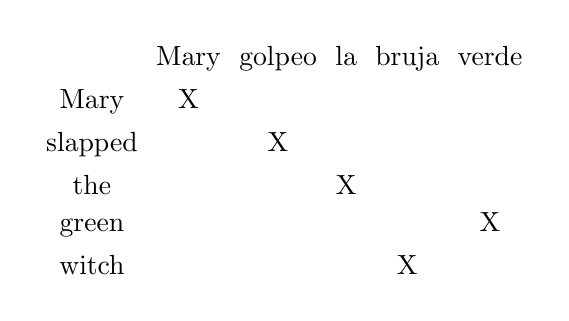
\begin{tikzpicture}
    \matrix(dict)[matrix of nodes, ampersand replacement=\&]{
      \ \& Mary \& golpeo \& la \& bruja \& verde \\
      Mary \& X \&  \&  \&  \&  \\
      slapped \&  \& X \&  \&  \&  \\
      the \&  \&  \&  X\&  \&  \\
      green \&  \&  \&  \&  \& X \\
      witch \&  \&  \&  \& X  \&  \\
    };
    \end{tikzpicture}
  \end{center}
\end{frame}



\begin{frame}{Hard Alignments}
  \begin{itemize}
  \item Have source vectors $\bolds_j^t$ 

    \air
  \item Could find greedy alignment at each step.
    \air
  \item Idea: learn scoring MLP, and use best aligned vector. 

  \item   At generation position $i$, For all source positions $j$, 
  \end{itemize}

  \[ z_j = \tanh( [ \bolds^t_i,  \bolds^s_j ] \boldW + \boldb)   \] 
  \[ j = \argmax_{j} z_j \]
  \[ w^t_{i+1} = \argmax_{w} O(w, \bolds^t_{i+1}, \bolds^s_j)  \] 

  What is the issue here?

\end{frame}



\begin{frame}{Attention: Soft Alignments}



  At generation position $i$, For all source positions $j$, 
  \[ z_j = \tanh( [ \bolds^t_i,  \bolds^s_j ] \boldW + \boldb)   \] 
  \[ \balpha = \softmax(\boldz) \] 

  \[ \boldc = \sum_{j} \alpha_j \bolds^s_j \] 
  \[ w^t_{i+1} = \argmax_{w} O(w, \bolds^t_{i+1}, \boldc)  \] 
  \air 

  \begin{itemize}
  \item $\alpha_j$ is the ``attention'' paid to source position $j$
  \end{itemize}
\end{frame}


\begin{frame}
  \begin{center}
    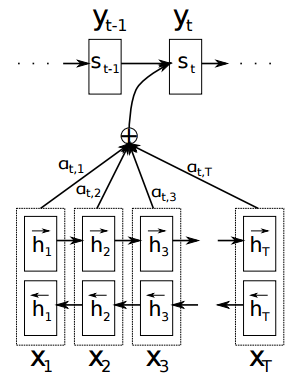
\includegraphics[width=5cm]{attenstruct}
  \end{center}
\end{frame}

\begin{frame}
  \begin{center}
    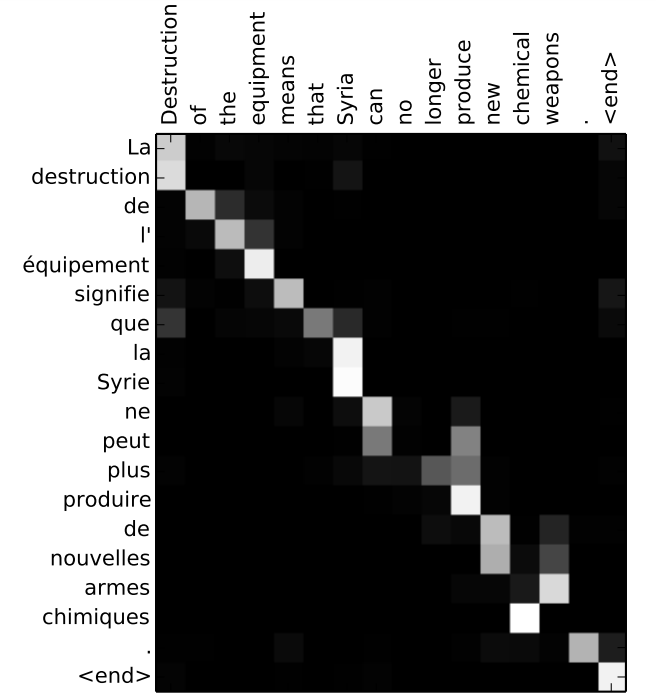
\includegraphics[width=0.6\textwidth]{attenalign}
  \end{center}
\end{frame}

\begin{frame}
  \begin{center}
    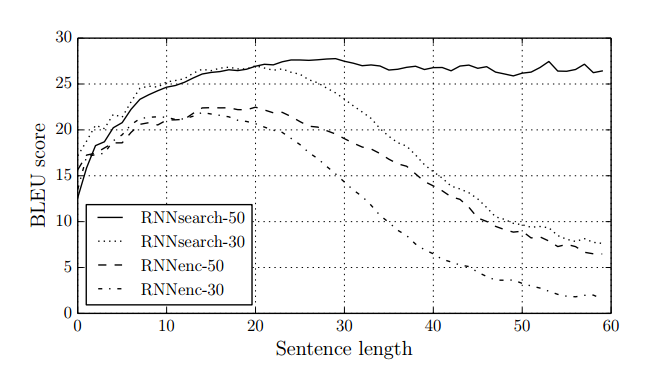
\includegraphics[width=0.6\textwidth]{attengraph}
  \end{center}
\end{frame}




% \begin{frame}{Argmax }
%   Can't backprop over the argmax 
%   \begin{center}
    
%   \end{center}
% \end{frame}

% \begin{frame}{The Attention Mechanism}
%   Idea: Replace internal argmax with softmax 

%   \begin{itemize}
%   \item Similar to the 
%   \end{itemize}
% \end{frame}

\begin{frame}
  \begin{quote}
    While the LSTM is capable of solving problems with long term
    dependencies, we discovered that the LSTM learns much better when
    the source sentences are reversed (the target sentences are not
    reversed). By doing so, the LSTM’s test perplexity dropped from
    5.8 to 4.7, and the test BLEU scores of its decoded translations
    increased from 25.9 to 30.6.
  \end{quote}
\end{frame}

% \begin{frame}{Attention-Based Encoder-Decoder}
%   At timestep $i$, 
 
%   \[\hat{\bolda} = \softmax(\boldS^s  \bolds^t_i ) \] 

%   Soft-alignment over source. 

%   \[p(a = | \boldx)  =\hat{\bolda}_i \]
% \end{frame}


\begin{frame}
  \begin{quote}
    We use a minibatch stochastic gradient descent (SGD) algorithm
    together with Adadelta (Zeiler, 2012) to train each model. Each
    SGD update direction is computed using a minibatch of 80
    sentences.  We trained each model for approximately 5 days.  Once
    a model is trained, we use a beam search to find a translation
    that approximately maximizes the conditional probability (see,
    e.g., Graves, 2012; Boulanger-Lewandowski et al., 2013). Sutskever
    et al. (2014) used this approach to generate translations from
    their neural machine translation model.
  \end{quote}
\end{frame}


\begin{frame}
  \begin{quote}
    WMT ’14 contains the following English-French parallel corpora: Europarl (61M words), news
commentary (5.5M), UN (421M) and two crawled corpora of 90M and 272.5M words respectively,
totaling 850M words. Following the procedure described in Cho et al. (2014a), we reduce the size of
the combined corpus to have 348M words using the data selection method by Axelrod et al. (2011).5
We do not use any monolingual data other than the mentioned parallel corpora, although it may be
possible to use a much larger monolingual corpus to pretrain an encoder.
  \end{quote}
\end{frame}




\end{document}